% Provenance (never printed): cycle 4 SVT, "La planete Terre": the dynamics of
% the Earth's outer shell, plates and their boundaries, continental drift as a
% history of ideas; see sources/outline_sources.md. Pilot chapter, 2026-10-22.
\chapter{La tectónica de placas: el rompecabezas que se mueve}\label{ch:g7:plate-tectonics}

Extiende un \omterm{def:g3:continents-and-oceans:world-map}{mapamundi} sobre una mesa y mira las dos orillas del \omterm{def:g2:water-on-earth:ocean}{océano}
Atlántico. La gran joroba de Brasil parece hecha para encajar en el hueco
de la \omterm{def:g1:landscapes-around-us:water}{costa} oeste de África, como si alguien hubiera cortado en dos un solo
trozo de tierra y hubiera separado las mitades. Los primeros que imprimieron
buenos \omterm{def:g2:drawing-to-map:map}{mapas} de las dos \omterm{def:g1:landscapes-around-us:water}{costas} se dieron cuenta enseguida. Durante tres
siglos siguió siendo una curiosidad. En el siglo~XX se convirtió en el punto
de partida de la teoría que hoy explica por qué tiembla el suelo en Japón,
por qué los Andes son tan altos, por qué Islandia se ensancha poco a poco
--- y por qué el \omterm{def:g2:drawing-to-map:map}{mapa} de la mesa no es más que una instantánea de un mundo
que se mueve.

\begin{omfigure}
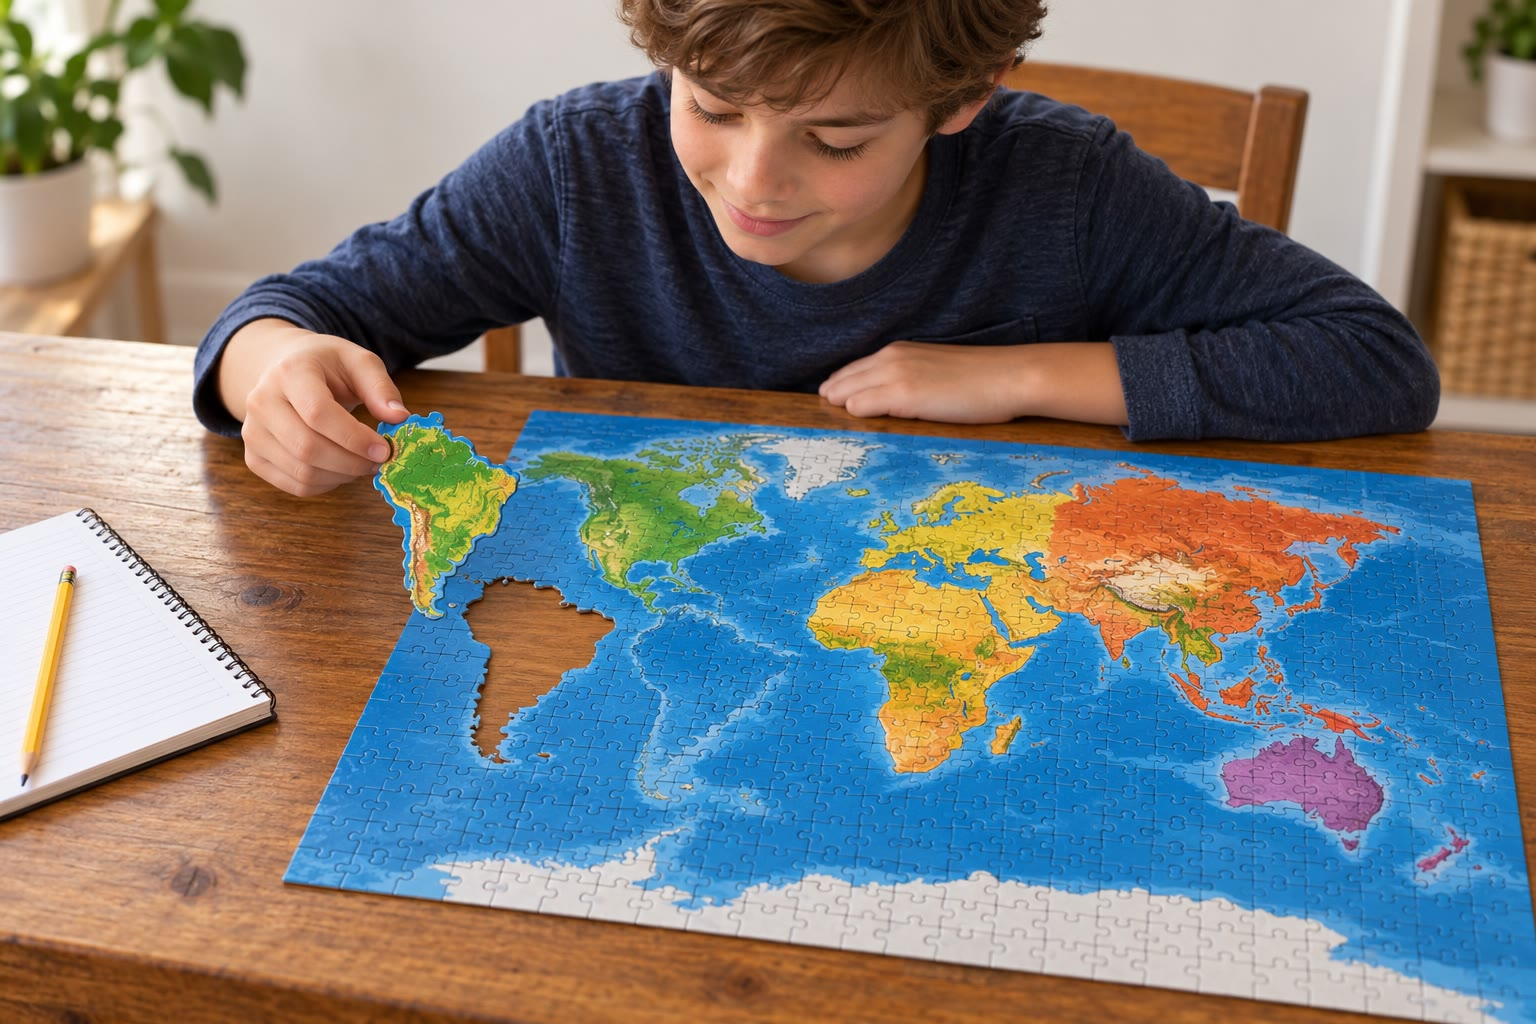
\includegraphics[width=0.62\linewidth]{images/book1/ai/g7-puzzle-map.jpg}

{\small América del Sur junto a África: en un rompecabezas, el encaje es un
juego; en la Tierra real, es una pista.}
\end{omfigure}

\begin{recall}
La Tierra tiene tres capas principales: una \emph{\omterm{def:g6:inside-the-earth:layers}{corteza}} fina y rocosa,
un \emph{\omterm{def:g6:inside-the-earth:layers}{manto}} grueso de \omterm{def:g3:stones-pebbles-sand:rock}{roca} caliente y un \emph{\omterm{def:g6:inside-the-earth:layers}{núcleo}} metálico; la
temperatura sube con la profundidad (\cref{ch:g6:inside-the-earth}). Un
lugar del \omterm{def:g3:continents-and-oceans:globe}{globo} se sitúa por su \omterm{def:g6:latitude-longitude:latitude}{latitud} y su \omterm{def:g6:latitude-longitude:longitude}{longitud}
(\cref{ch:g6:latitude-longitude}).
\end{recall}

\section{Continentes que antes encajaban}

\begin{definition}[Deriva continental]\label{def:g7:plate-tectonics:continental-drift}
La \emph{deriva continental}\index{deriva continental} es la idea de que
los \omterm{def:g3:continents-and-oceans:continent}{continentes} se desplazan lentamente sobre la superficie de la Tierra,
de modo que sus posiciones, y la forma de los \omterm{def:g2:water-on-earth:ocean}{océanos} que hay entre ellos,
han cambiado a lo largo de las eras.
\end{definition}

\begin{definition}[Supercontinente]\label{def:g7:plate-tectonics:supercontinent}
Un \emph{supercontinente}\index{supercontinente} es una sola masa de tierra
formada por todos los \omterm{def:g3:continents-and-oceans:continent}{continentes}, o casi todos, unidos. El último,
\emph{Pangea}\index{Pangea} (``todas las tierras'' en griego), empezó a
fragmentarse hace entre unos 225 y 200 millones de años.
% ledger: usgs:pangaea-breakup
\end{definition}

El científico que defendió la \omterm{def:g7:plate-tectonics:continental-drift}{deriva continental} como una teoría de
verdad, con pruebas, fue Alfred Wegener. Reunió cuatro clases de pistas.

\begin{enumerate}
  \item \textbf{La forma de las \omterm{def:g1:landscapes-around-us:water}{costas}.} América del Sur y África encajan
        como dos piezas de un rompecabezas, y lo mismo ocurre con otras
        \omterm{def:g1:landscapes-around-us:water}{costas}.
  \item \textbf{Los fósiles.} Los mismos animales y plantas fósiles se
        encuentran en \omterm{def:g3:continents-and-oceans:continent}{continentes} que hoy están separados por miles de
        kilómetros de \omterm{def:g2:water-on-earth:ocean}{océano}. \emph{Mesosaurus} era un pequeño reptil que
        vivía en \omterm{def:g2:water-on-earth:salt-fresh}{agua dulce}: no podía cruzar un \omterm{def:g2:water-on-earth:ocean}{océano} a nado, y sin embargo
        sus fósiles están a la vez en Brasil y en el sur de África.
  \item \textbf{Las \omterm{def:g3:stones-pebbles-sand:rock}{rocas}.} \omterm{def:g3:stones-pebbles-sand:rock}{Rocas} de las mismas clases y edades, y antiguas
        \omterm{def:g4:world-physical-map:range}{cordilleras} de la misma forma, se interrumpen en una \omterm{def:g1:landscapes-around-us:water}{costa} y vuelven
        a empezar en la opuesta, como las líneas impresas de un periódico
        roto.
  \item \textbf{Los \omterm{def:g5:weather-and-climate:climate}{climas} antiguos.} En la Antártida hay carbón, hecho con
        las plantas de bosques pantanosos y cálidos; en zonas de África que
        hoy son cálidas y secas hay huellas dejadas por antiguos glaciares.
        Estas tierras tuvieron que estar en otro tiempo en otros \omterm{def:g5:weather-and-climate:climate}{climas}, en
        otras \omterm{def:g6:latitude-longitude:latitude}{latitudes}.
\end{enumerate}
% ledger: usgs:coal-antarctica, usgs:fossil-map

\begin{omfigure}
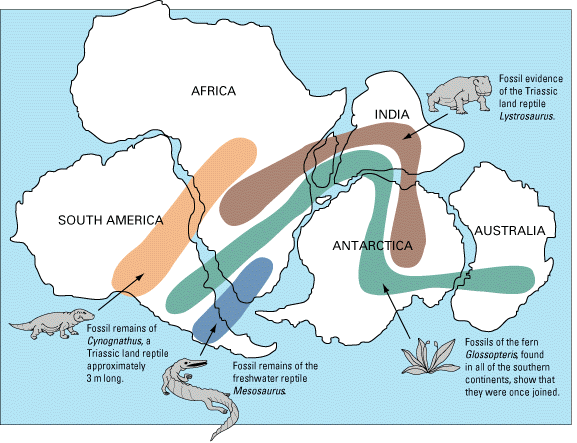
\includegraphics[width=0.86\linewidth]{images/book1/g7-usgs-fossil-map.png}

{\small Los \omterm{def:g3:continents-and-oceans:continent}{continentes} del sur, vueltos a juntar. Cada franja de color une
los lugares donde se encuentra hoy una especie fósil: los reptiles
terrestres \emph{Cynognathus} y \emph{Lystrosaurus}, el reptil de \omterm{def:g2:water-on-earth:salt-fresh}{agua dulce}
\emph{Mesosaurus} y el helecho \emph{Glossopteris}. Separados, los
\omterm{def:g3:continents-and-oceans:continent}{continentes} dispersan las franjas; juntos, las franjas siguen sin cortes.
\omterm{def:g2:drawing-to-map:map}{Mapa}: U.S. Geological Survey, \emph{This Dynamic Earth} (dominio público).}
\end{omfigure}

\begin{history}[La idea de Wegener, 1912--1930]
% ledger: usgs:wegener-1912, usgs:wegener-death, usgs:jeffreys
Alfred Wegener, un meteorólogo alemán de 32 años, expuso la teoría de la
\omterm{def:g7:plate-tectonics:continental-drift}{deriva continental} en dos artículos en 1912. La mayoría de los geólogos la
rechazaron. La objeción más fuerte era que Wegener no podía decir \emph{qué}
movía los \omterm{def:g3:continents-and-oceans:continent}{continentes}: pensaba que avanzaban abriéndose paso a través de la
\omterm{def:g3:stones-pebbles-sand:rock}{roca} del fondo del \omterm{def:g2:water-on-earth:ocean}{océano}, y el físico Harold Jeffreys demostró que unos
\omterm{def:g3:continents-and-oceans:continent}{continentes} sólidos no podían hacer eso sin romperse. Wegener siguió
reuniendo pruebas hasta que murió en el inlandsis de Groenlandia en
1930, durante una expedición. La respuesta que le faltaba vino del fondo de
los \omterm{def:g2:water-on-earth:ocean}{océanos}, explorado a partir de la década de 1950: se cuenta en un curso
posterior.
\end{history}

\section{Las placas}

Las pistas de Wegener eran correctas, pero sus \omterm{def:g3:continents-and-oceans:continent}{continentes} no eran las
piezas adecuadas. No solo se mueven los \omterm{def:g3:continents-and-oceans:continent}{continentes}: toda la envoltura
exterior de la Tierra, tanto bajo los \omterm{def:g3:continents-and-oceans:continent}{continentes} como bajo los \omterm{def:g2:water-on-earth:ocean}{océanos},
está rota en pedazos.

\begin{definition}[Placa tectónica]\label{def:g7:plate-tectonics:plate}
Una \emph{placa tectónica}\index{placa tectonica@placa tectónica} (o
simplemente una placa) es una gran losa rígida de \omterm{def:g3:stones-pebbles-sand:rock}{roca} que forma parte de
la envoltura exterior de la Tierra. Una placa está formada por la \omterm{def:g6:inside-the-earth:layers}{corteza} y
por la parte más alta del \omterm{def:g6:inside-the-earth:layers}{manto}, fría y rígida, con un espesor total de al
menos 80 kilómetros de media; se desplaza lentamente sobre el \omterm{def:g6:inside-the-earth:layers}{manto} más
caliente y más blando que tiene debajo.
% ledger: usgs:lithosphere-80km
\end{definition}

\begin{definition}[Tectónica de placas]\label{def:g7:plate-tectonics:plate-tectonics}
La \emph{tectónica de placas}\index{tectonica de placas@tectónica de placas}
es la teoría según la cual la envoltura exterior de la Tierra está dividida
en \omterm{def:g7:plate-tectonics:plate}{placas} que se mueven unas respecto a otras, y la mayoría de los
\omterm{def:g4:volcanoes-earthquakes-first-look:earthquake}{terremotos}, los \omterm{def:g4:volcanoes-earthquakes-first-look:volcano}{volcanes} y las \omterm{def:g4:world-physical-map:range}{cordilleras} se producen donde se encuentran
las \omterm{def:g7:plate-tectonics:plate}{placas}.
\end{definition}

\begin{remark}[¿Cuántas placas?]\label{rem:g7:plate-tectonics:how-many}
% ledger: usgs:plates-dozen, pb2002:count
Una docena de \omterm{def:g7:plate-tectonics:plate}{placas}, más o menos, son grandes; muchas más son pequeñas. Un
\omterm{def:g2:drawing-to-map:map}{mapa} detallado que usan los geólogos cuenta 52. Una \omterm{def:g7:plate-tectonics:plate}{placa} puede llevar un
\omterm{def:g3:continents-and-oceans:continent}{continente}, un \omterm{def:g2:water-on-earth:ocean}{océano} o las dos cosas: la \omterm{def:g7:plate-tectonics:plate}{placa} Sudamericana lleva toda
América del Sur y la mitad occidental del Atlántico Sur. La \omterm{def:g7:plate-tectonics:plate}{placa} del
Pacífico, la más grande, casi no lleva tierra firme.
\end{remark}

\begin{omfigure}
\begin{tikzpicture}
\begin{axis}[ommap, width=\linewidth, xtick={-180,-90,...,180}, ytick={-60,0,60}]
\addplot[fill=omLithAlluv, draw=black!45, line width=0.2pt] table {figdata/out/shared-geo-land.dat};
\addplot[omRidge, line width=0.8pt] table {figdata/out/shared-geo-school-ridge.dat};
\addplot[omRidge!70!black, line width=0.8pt] table {figdata/out/shared-geo-school-transform.dat};
\addplot[omTrench, line width=0.8pt] table {figdata/out/shared-geo-school-subduction.dat};
\addplot[fill=omTrench, draw=none] table {figdata/out/shared-geo-school-teeth.dat};
\addplot[black!65, line width=0.8pt] table {figdata/out/shared-geo-school-collision.dat};
\begin{scope}[every node/.style={font=\scriptsize\bfseries, text=black!85,
    fill=white, fill opacity=0.75, text opacity=1, inner sep=1pt, align=center}]
  \node at (axis cs:-150,12) {Pacífica};
  \node at (axis cs:-103,52) {Norte-\\americana};
  \node at (axis cs:-48,-12) {Sud-\\americana};
  \node at (axis cs:85,57) {Euroasiática};
  \node at (axis cs:18,8) {Africana};
  \node at (axis cs:10,-75) {Antártica};
  \node at (axis cs:78,11) {Índica};
  \node at (axis cs:128,-26) {Australiana};
  \node at (axis cs:-95,-22) {de Nazca};
  \node at (axis cs:50,20) {Arábiga};
\end{scope}
\end{axis}
\end{tikzpicture}

{\small Las principales \omterm{def:g7:plate-tectonics:plate}{placas tectónicas}. En rojo, \omterm{def:g7:plate-tectonics:plate}{placas} que se separan;
en azul con triángulos, una \omterm{def:g7:plate-tectonics:plate}{placa} que se hunde bajo la otra (los triángulos
están en la \omterm{def:g7:plate-tectonics:plate}{placa} que queda encima); en gris, \omterm{def:g7:plate-tectonics:plate}{placas} que se empujan a lo
largo de una ancha zona de \omterm{def:g1:landscapes-around-us:landform}{montañas}; en rojo oscuro, \omterm{def:g7:plate-tectonics:plate}{placas} que se deslizan
una junto a otra. Límites según P.~Bird (2003); \omterm{def:g1:landscapes-around-us:water}{costas} de Natural Earth.}
\end{omfigure}

¿Cómo sabemos dónde acaba una \omterm{def:g7:plate-tectonics:plate}{placa} y empieza la siguiente? Fijándonos en
los lugares donde la Tierra no está quieta.

\begin{proposition}[Los terremotos y los volcanes dibujan los límites de las placas]\label{prop:g7:plate-tectonics:restless}
% ledger: data:usgs-comcat, data:pb2002 (share computed in figdata/grade-7/quakes_on_boundaries.py)
Los \omterm{def:g4:volcanoes-earthquakes-first-look:earthquake}{terremotos} y los \omterm{def:g4:volcanoes-earthquakes-first-look:volcano}{volcanes} no están repartidos al azar por la Tierra: la
mayoría se sitúan a lo largo de franjas estrechas, y esas franjas son los
bordes de las \omterm{def:g7:plate-tectonics:plate}{placas}. De los 7\,031 \omterm{def:g4:volcanoes-earthquakes-first-look:earthquake}{terremotos} de magnitud 6 o más
registrados entre 1976 y 2025, 6\,472 --- es decir, el 92\,\% --- ocurrieron
a menos de \qty{300}{km} de un \omterm{def:g7:plate-tectonics:plate-boundary}{límite de placas}.
\end{proposition}

\begin{omfigure}
\begin{tikzpicture}
\begin{axis}[ommap, width=\linewidth, xtick={-180,-90,...,180}, ytick={-60,0,60},
  legend style={at={(0.02,0.04)}, anchor=south west, font=\scriptsize,
  fill=white, fill opacity=0.85, text opacity=1, draw=black!40}]
\addplot[fill=omLithAlluv, draw=black!45, line width=0.2pt, forget plot] table {figdata/out/shared-geo-land.dat};
\addplot[only marks, mark=*, mark size=0.45pt, omThm!85!black] table[x=lon, y=lat] {figdata/out/grade-7-quakes_on_boundaries-map.dat};
\addlegendentry{terremoto de magnitud 6.5 o más, 1976--2025}
\addplot[only marks, mark=triangle*, mark size=1.1pt, black] table {figdata/out/shared-geo-volcanoes.dat};
\addlegendentry{volcán activo en los últimos 12\,000 años}
\end{axis}
\end{tikzpicture}

{\small Los grandes \omterm{def:g4:volcanoes-earthquakes-first-look:earthquake}{terremotos} y los \omterm{def:g4:volcanoes-earthquakes-first-look:volcano}{volcanes} recientes. Compáralo con el
\omterm{def:g2:drawing-to-map:map}{mapa} de las \omterm{def:g7:plate-tectonics:plate}{placas} de arriba: los puntos y los triángulos dibujan los
límites de las \omterm{def:g7:plate-tectonics:plate}{placas}. Datos: catálogo de \omterm{def:g4:volcanoes-earthquakes-first-look:earthquake}{terremotos} del U.S. Geological
Survey; Global Volcanism Program de la Smithsonian.}
\end{omfigure}

\section{Tres clases de límites de placas}

\begin{definition}[Límite de placas]\label{def:g7:plate-tectonics:plate-boundary}
Un \emph{límite de placas}\index{limite de placas@límite de placas} es la
línea, o la zona estrecha, donde se encuentran dos \omterm{def:g7:plate-tectonics:plate}{placas}. Según cómo se
mueven las dos \omterm{def:g7:plate-tectonics:plate}{placas} una respecto a la otra, un límite es de una de estas
tres clases:
\begin{itemize}
  \item en un \emph{límite divergente}\index{limite divergente@límite divergente}
        las dos \omterm{def:g7:plate-tectonics:plate}{placas} se separan;
  \item en un \emph{límite convergente}\index{limite convergente@límite convergente}
        las dos \omterm{def:g7:plate-tectonics:plate}{placas} se acercan;
  \item en un \emph{límite transformante}\index{limite transformante@límite transformante}
        las dos \omterm{def:g7:plate-tectonics:plate}{placas} se deslizan una junto a otra, lado a lado.
\end{itemize}
\end{definition}

\begin{example}[Límites divergentes: Islandia y el este de África]\label{ex:g7:plate-tectonics:divergent}
% ledger: usgs:iceland, usgs:east-africa
Por el centro del \omterm{def:g2:water-on-earth:ocean}{océano} Atlántico corre una cadena de \omterm{def:g1:landscapes-around-us:landform}{montañas} submarinas,
la dorsal mesoatlántica, donde las \omterm{def:g7:plate-tectonics:plate}{placas} de los dos lados se separan. La
\omterm{def:g3:stones-pebbles-sand:rock}{roca} caliente del \omterm{def:g6:inside-the-earth:layers}{manto} sube hacia el hueco, se funde en parte y se
convierte en nuevo fondo marino: un \omterm{def:g7:plate-tectonics:plate-boundary}{límite divergente} fabrica \omterm{def:g7:plate-tectonics:plate}{placa} nueva.
Islandia es un trozo de esta dorsal que asoma por encima del \omterm{def:g2:water-on-earth:ocean}{mar}: allí,
América del Norte se desplaza hacia el oeste y Eurasia hacia el este, y la
isla se va abriendo lentamente. Entre 1975 y 1984, las grietas cercanas al
\omterm{def:g4:volcanoes-earthquakes-first-look:volcano}{volcán} Krafla, en el norte de la isla, se ensancharon unos 7 metros en
total. Un \omterm{def:g7:plate-tectonics:plate-boundary}{límite divergente} también puede atravesar un \omterm{def:g3:continents-and-oceans:continent}{continente}: a lo
largo del rift de África Oriental, África empieza a partirse, y el \omterm{def:g2:water-on-earth:ocean}{mar} Rojo
es un \omterm{def:g2:water-on-earth:ocean}{océano} joven que ya ha separado Arabia de África.
\end{example}

\begin{example}[Límites convergentes: los Andes y el Himalaya]\label{ex:g7:plate-tectonics:convergent}
% ledger: usgs:trench-depth, usgs:himalaya
Frente a la \omterm{def:g1:landscapes-around-us:water}{costa} oeste de América del Sur, la \omterm{def:g7:plate-tectonics:plate}{placa} de Nazca, que lleva
\omterm{def:g2:water-on-earth:ocean}{océano}, se acerca a la \omterm{def:g7:plate-tectonics:plate}{placa} Sudamericana, que lleva un \omterm{def:g3:continents-and-oceans:continent}{continente}. La \omterm{def:g7:plate-tectonics:plate}{placa}
oceánica, más pesada, se dobla y se hunde bajo el \omterm{def:g3:continents-and-oceans:continent}{continente}, hasta lo hondo
del \omterm{def:g6:inside-the-earth:layers}{manto}. A lo largo de la línea por donde baja, el fondo marino se
precipita en una fosa profunda; por encima de la \omterm{def:g7:plate-tectonics:plate}{placa} que se hunde, la
tierra se ve sacudida por \omterm{def:g4:volcanoes-earthquakes-first-look:earthquake}{terremotos} y bordeada de \omterm{def:g4:volcanoes-earthquakes-first-look:volcano}{volcanes}: los Andes. En
el oeste del Pacífico, donde una \omterm{def:g7:plate-tectonics:plate}{placa} oceánica se hunde bajo otra, las
fosas son los lugares más profundos de la Tierra: la fosa de las Marianas
tiene casi \qty{11000}{m} de profundidad. Cuando se encuentran dos
\omterm{def:g3:continents-and-oceans:continent}{continentes}, ninguno se hunde: la \omterm{def:g6:inside-the-earth:layers}{corteza} se arruga y se engrosa. La India
chocó con Asia hace unos 50 millones de años, y las dos \omterm{def:g7:plate-tectonics:plate}{placas} siguen
empujando; así se levantaron el Himalaya y la meseta del Tíbet.
\end{example}

\begin{example}[Un límite transformante: la falla de San Andrés]\label{ex:g7:plate-tectonics:transform}
% ledger: usgs:san-andreas, usgs:san-andreas-photo
En California, la \omterm{def:g7:plate-tectonics:plate}{placa} del Pacífico se desliza hacia el noroeste junto a
la \omterm{def:g7:plate-tectonics:plate}{placa} Norteamericana a lo largo de la falla de San Andrés, de unos
\qty{1300}{km} de longitud. Allí no se fabrica ni se destruye \omterm{def:g7:plate-tectonics:plate}{placa}; las
dos \omterm{def:g7:plate-tectonics:plate}{placas} rozan una contra otra, y las sacudidas de ese roce son
\omterm{def:g4:volcanoes-earthquakes-first-look:earthquake}{terremotos}.
\end{example}

\begin{omfigure}
\begin{tikzpicture}[x=1cm, y=1cm, font=\small]
  % mantle
  \fill[omLithGranite!45] (0,-3.3) rectangle (12.4,-0.85);
  \node[font=\footnotesize, text=black!75] at (2.6,-2.6) {manto: caliente y blando};
  % sea water
  \fill[omSea] (0,0) -- (0,-0.75) -- (1.5,-0.6) -- (3,-0.25) -- (4.5,-0.6)
    -- (7.4,-0.8) -- (8.0,-1.2) -- (8.6,-0.6) -- (8.9,0) -- cycle;
  % oceanic plates (the ridge at x = 3, the trench at x = 8)
  \fill[omLithBasalt!70] (0,-0.75) -- (1.5,-0.6) -- (3,-0.25) -- (4.5,-0.6)
    -- (7.4,-0.8) -- (8.0,-1.2) -- (9.6,-2.3) -- (10.2,-3.3) -- (9.5,-3.3)
    -- (8.6,-2.2) -- (7.5,-1.55) -- (4.5,-1.35) -- (3.2,-0.95) -- (2.8,-0.95)
    -- (1.5,-1.35) -- (0,-1.45) -- cycle;
  % continental plate
  \fill[omLithSand!80] (8.6,-0.6) -- (8.9,0) -- (9.4,0.35) -- (9.8,0.9)
    -- (10.2,0.35) -- (12.4,0.2) -- (12.4,-1.9) -- (10.6,-1.9) -- (9.6,-2.3)
    -- (8.0,-1.2) -- cycle;
  \draw[black!70, line width=0.5pt] (0,-0.75) -- (1.5,-0.6) -- (3,-0.25)
    -- (4.5,-0.6) -- (7.4,-0.8) -- (8.0,-1.2) -- (8.6,-0.6) -- (8.9,0)
    -- (9.4,0.35) -- (9.8,0.9) -- (10.2,0.35) -- (12.4,0.2);
  \draw[black!45, densely dashed] (0,0) -- (8.9,0);
  % magma: under the ridge and under the volcano
  \fill[omThm!80] (2.85,-0.95) -- (3,-0.3) -- (3.15,-0.95) -- cycle;
  \draw[omThm!80, line width=1.4pt, -{Stealth[length=2.2mm]}] (3,-1.85) -- (3,-1.0);
  \draw[omThm!80, line width=1.2pt, decorate, decoration={snake, amplitude=0.6pt,
    segment length=4pt}] (9.8,-2.45) -- (9.8,0.75);
  % plate motions
  \draw[black, line width=1pt, -{Stealth[length=2.4mm]}] (2.5,-0.75) -- (1.3,-0.95);
  \draw[black, line width=1pt, -{Stealth[length=2.4mm]}] (3.5,-0.75) -- (5.4,-1.05);
  \draw[black, line width=1pt, -{Stealth[length=2.4mm]}] (12.1,-0.85) -- (10.9,-0.85);
  \draw[black, line width=1pt, -{Stealth[length=2.4mm]}] (8.7,-1.75) -- (9.3,-2.25);
  % labels
  \node[font=\footnotesize, align=center, above] at (3,0.05) {límite divergente:\\dorsal oceánica};
  \node[font=\footnotesize, align=center, below] at (6.9,-1.95) {límite convergente:\\la placa oceánica se hunde};
  \draw[black!60, thin] (8.0,-1.25) -- (7.6,-1.9);
  \node[font=\footnotesize, above] at (8.0,0.05) {fosa};
  \draw[black!60, thin] (8.0,0.05) -- (8.0,-1.1);
  \node[font=\footnotesize, above] at (9.8,0.95) {volcán};
  \node[font=\footnotesize] at (11.4,-0.4) {continente};
  \node[font=\footnotesize] at (1.2,-1.6) {placa oceánica};
  \node[font=\footnotesize, text=black!70] at (5.6,-0.32) {océano};
\end{tikzpicture}

\medskip
\begin{tikzpicture}[font=\small]
  \fill[omLithBasalt!45] (0,0) rectangle (2.4,2.2);
  \fill[omLithSand!70] (2.4,0) rectangle (4.8,2.2);
  \draw[fault] (2.4,-0.1) -- (2.4,2.3);
  \draw[black, line width=1pt, -{Stealth[length=2.4mm]}] (1.2,0.5) -- (1.2,1.7);
  \draw[black, line width=1pt, -{Stealth[length=2.4mm]}] (3.6,1.7) -- (3.6,0.5);
  \node[font=\footnotesize, below] at (1.2,-0.1) {placa A};
  \node[font=\footnotesize, below] at (3.6,-0.1) {placa B};
  \node[font=\footnotesize, align=left, anchor=west] at (5.1,1.1)
    {límite transformante, visto desde arriba:\\las placas se deslizan una junto a otra;\\no se fabrica ni se destruye placa};
\end{tikzpicture}

{\small Arriba, un corte a través de dos \omterm{def:g7:plate-tectonics:plate-boundary}{límites de placas} (no a escala;
las profundidades están muy exageradas). En la dorsal, las \omterm{def:g7:plate-tectonics:plate}{placas} se
separan y sube \omterm{def:g3:stones-pebbles-sand:rock}{roca} caliente del \omterm{def:g6:inside-the-earth:layers}{manto}; en la fosa, la \omterm{def:g7:plate-tectonics:plate}{placa} oceánica se
hunde bajo el \omterm{def:g3:continents-and-oceans:continent}{continente}, y la \omterm{def:g3:stones-pebbles-sand:rock}{roca} que se funde por encima de ella
alimenta \omterm{def:g4:volcanoes-earthquakes-first-look:volcano}{volcanes}. Abajo, un \omterm{def:g7:plate-tectonics:plate-boundary}{límite transformante} visto desde arriba.}
\end{omfigure}

\begin{omfigure}
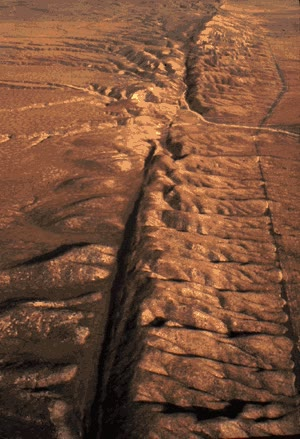
\includegraphics[width=0.28\linewidth]{images/book1/g7-usgs-san-andreas.jpg}

{\small La falla de San Andrés cruzando la \omterm{def:g1:landscapes-around-us:landform}{llanura} de Carrizo, en
California, vista desde un avión: el largo \omterm{def:g1:landscapes-around-us:landform}{valle} recto es el límite entre
la \omterm{def:g7:plate-tectonics:plate}{placa} del Pacífico (a la izquierda) y la \omterm{def:g7:plate-tectonics:plate}{placa} Norteamericana (a la
derecha). Fotografía: Robert E. Wallace, U.S. Geological Survey (dominio
público).}
\end{omfigure}

\begin{method}[Reconocer un límite de placas en un mapa]\label{met:g7:plate-tectonics:recognise}
Para decidir qué clase de límite separa dos \omterm{def:g7:plate-tectonics:plate}{placas}:
\begin{enumerate}
  \item busca, en un \omterm{def:g2:drawing-to-map:map}{mapa} de los movimientos de las \omterm{def:g7:plate-tectonics:plate}{placas}, las flechas de
        los dos lados del límite;
  \item si se alejan del límite, es divergente; si apuntan hacia él,
        convergente; si son paralelas a él y apuntan en sentidos opuestos,
        transformante;
  \item compruébalo con el \omterm{def:g1:landscapes-around-us:landscape}{paisaje}: una dorsal en medio de un \omterm{def:g2:water-on-earth:ocean}{océano} o un
        rift que atraviesa un \omterm{def:g3:continents-and-oceans:continent}{continente} van con un \omterm{def:g7:plate-tectonics:plate-boundary}{límite divergente}; una
        fosa profunda con una línea de \omterm{def:g4:volcanoes-earthquakes-first-look:volcano}{volcanes}, o una alta \omterm{def:g4:world-physical-map:range}{cordillera}, con
        uno convergente; una larga falla recta sin ninguna de las dos cosas,
        con un \omterm{def:g7:plate-tectonics:plate-boundary}{límite transformante}.
\end{enumerate}
\end{method}

\section{¿A qué velocidad se mueven las placas?}

\begin{proposition}[Unos pocos centímetros al año]\label{prop:g7:plate-tectonics:speed}
% ledger: data:pb2002 (speeds computed in figdata/grade-7/plate_speeds.py), usgs:mar-rate
Dos \omterm{def:g7:plate-tectonics:plate}{placas} vecinas se mueven una respecto a la otra a una velocidad de unos
pocos centímetros al año: desde unos 2 centímetros al año a través del
Atlántico Norte hasta más de 14 centímetros al año a través de la dorsal
del Pacífico oriental, la dorsal que se abre más deprisa de la Tierra.
\end{proposition}

\begin{omfigure}
\begin{tikzpicture}
\begin{axis}[xbar, width=0.82\linewidth, height=5.4cm, xmin=0, xmax=16.5,
  ytick={1,...,6}, yticklabels={dorsal del Atlántico Norte, dorsal del Atlántico Sur,
  falla de San Andrés, Himalaya, fosa de Perú--Chile, dorsal del Pacífico oriental},
  y tick label style={font=\small}, tick label style={font=\small},
  xlabel={velocidad de una placa respecto a la otra (cm al año)},
  label style={font=\small}, bar width=7pt, axis x line=bottom,
  axis y line=left, axis line style={-}, enlarge y limits=0.12,
  nodes near coords, nodes near coords style={font=\scriptsize},
  every node near coord/.append style={/pgf/number format/fixed,
  /pgf/number format/precision=1, /pgf/number format/fixed zerofill}]
\addplot[fill=omDef!55, draw=omDef!80!black] table[x=speed_cm_a, y=rank] {figdata/out/grade-7-plate_speeds.dat};
\end{axis}
\end{tikzpicture}

{\small A qué velocidad se mueven las \omterm{def:g7:plate-tectonics:plate}{placas} en seis límites: medias a lo
largo de cada límite calculadas con el modelo de \omterm{def:g7:plate-tectonics:plate}{placas} de P.~Bird (2003).}
\end{omfigure}

\begin{method}[De centímetros al año a kilómetros por millón de años]\label{met:g7:plate-tectonics:convert}
Un kilómetro son \num{100000} centímetros. Una velocidad de \qty{1}{cm} al
año, mantenida durante un millón de años, recorre por tanto
\num{1000000} centímetros, es decir, \qty{10}{km}. Así pues:
\[
  1\ \text{cm al año} = 10\ \text{km por millón de años}.
\]
Multiplica una velocidad en centímetros al año por 10 para obtener
kilómetros por millón de años; después multiplica por un número de millones
de años para obtener una distancia en kilómetros, o divide una distancia
entre la velocidad para obtener un tiempo.
\end{method}

\begin{example}[El Atlántico crece]\label{ex:g7:plate-tectonics:atlantic}
% ledger: usgs:mar-rate
De media, los dos lados de la dorsal mesoatlántica se separan unos
\qty{2.5}{cm} al año, es decir, \qty{25}{km} por millón de años. En 100
millones de años, eso hace \qty{2500}{km}: mantenida el tiempo suficiente,
una velocidad demasiado lenta para notarla en toda una vida abre un \omterm{def:g2:water-on-earth:ocean}{océano}.
\end{example}

\begin{remark}[Medir el movimiento hoy]\label{rem:g7:plate-tectonics:gps}
% ledger: usgs:gps
Hoy estos movimientos tan lentos se miden directamente. Unas estaciones
permanentes, fijadas al \omterm{def:g3:stones-pebbles-sand:rock}{lecho rocoso}, reciben las señales de los satélites
de posicionamiento y calculan su propia posición, día tras día, con una
precisión de unos pocos milímetros. Al cabo de unos años, se ve que las
estaciones situadas en \omterm{def:g7:plate-tectonics:plate}{placas} distintas se alejan o se acercan, a las
velocidades halladas en las \omterm{def:g3:stones-pebbles-sand:rock}{rocas} a lo largo de millones de años. El propio
posicionamiento por satélite es el tema del \cref{ch:g9:maps-of-the-earth}.
\end{remark}

\begin{omfigure}
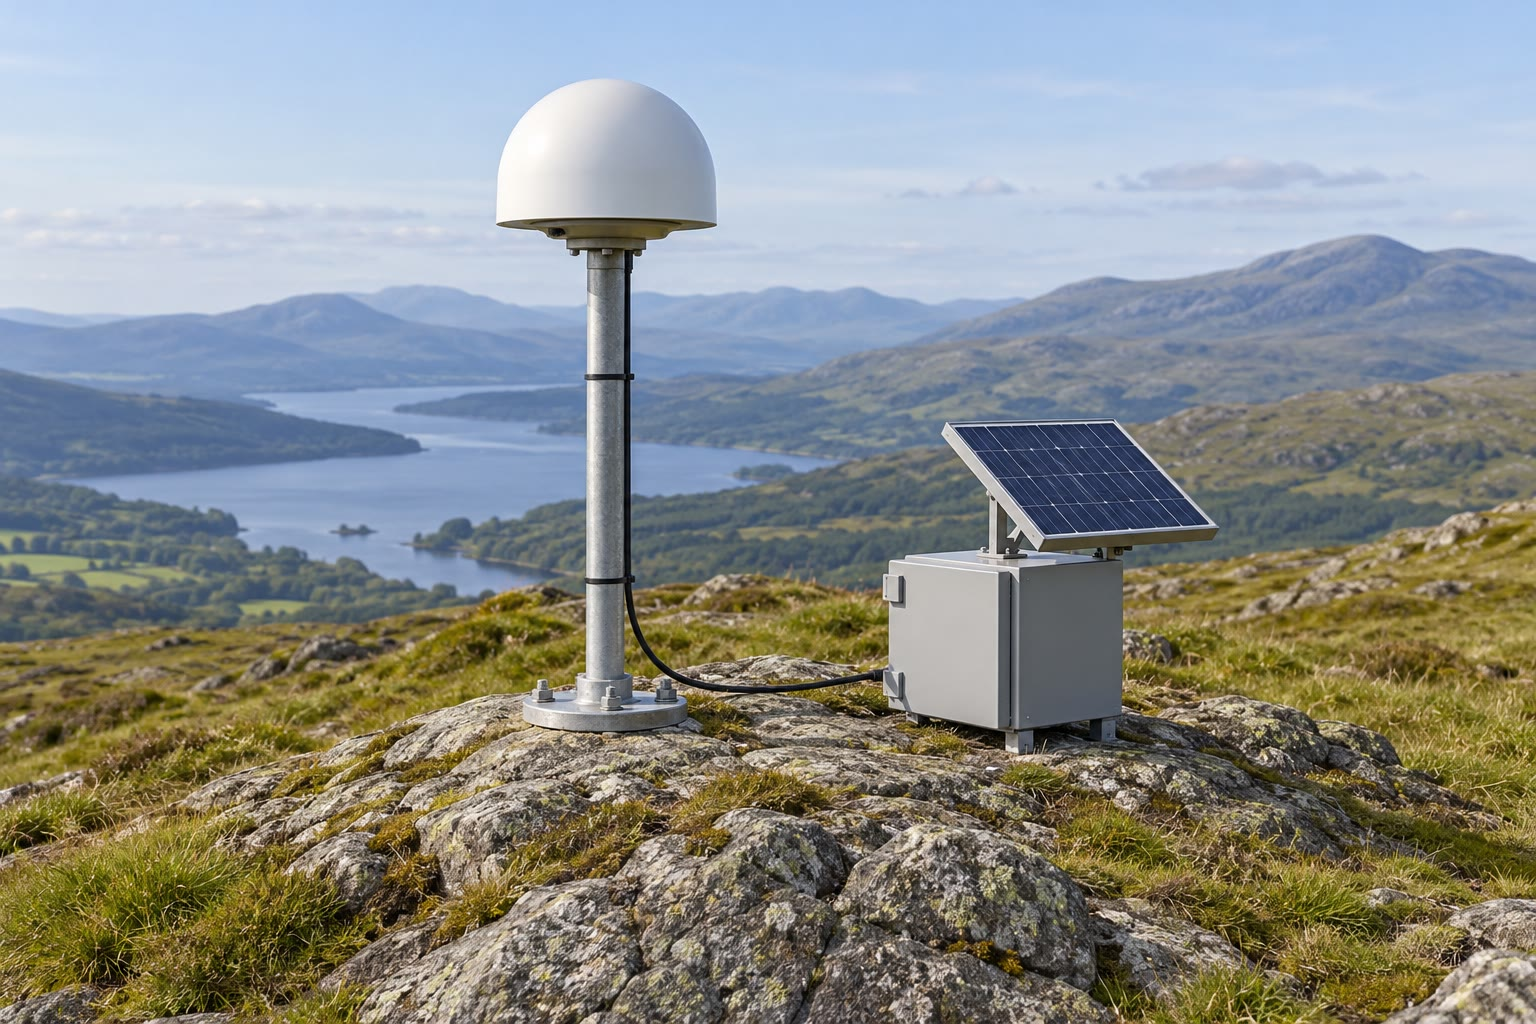
\includegraphics[width=0.55\linewidth]{images/book1/ai/g7-gps-station.jpg}

{\small Una estación permanente de posicionamiento: su antena está
atornillada a la \omterm{def:g3:stones-pebbles-sand:rock}{roca}, así que se mueve con la \omterm{def:g7:plate-tectonics:plate}{placa}.}
\end{omfigure}

\section{Ejercicios}

\begin{exercise}[$\star$]\label{exo:g7:plate-tectonics:1}
¿Qué es la \omterm{def:g7:plate-tectonics:continental-drift}{deriva continental}? Di las cuatro clases de pistas que usó
Wegener para defenderla.
\end{exercise}

\begin{exercise}[$\star$]\label{exo:g7:plate-tectonics:2}
Nombra las tres clases de \omterm{def:g7:plate-tectonics:plate-boundary}{límites de placas} y di, para cada una, cómo se
mueven las dos \omterm{def:g7:plate-tectonics:plate}{placas} una respecto a la otra.
\end{exercise}

\begin{exercise}[$\star$]\label{exo:g7:plate-tectonics:3}
Mira el \omterm{def:g2:drawing-to-map:map}{mapa} de los \omterm{def:g4:volcanoes-earthquakes-first-look:earthquake}{terremotos} y los \omterm{def:g4:volcanoes-earthquakes-first-look:volcano}{volcanes}. Nombra dos regiones del mundo
con muchos \omterm{def:g4:volcanoes-earthquakes-first-look:earthquake}{terremotos} grandes, y un \omterm{def:g3:continents-and-oceans:continent}{continente} que casi no tiene ninguno en
su interior.
\end{exercise}

\begin{exercise}[$\star$]\label{exo:g7:plate-tectonics:4}
En Brasil y en el sur de África se encuentran fósiles de \emph{Mesosaurus},
un pequeño reptil que vivía en \omterm{def:g2:water-on-earth:salt-fresh}{agua dulce}. ¿Por qué es esto una pista de que
los dos \omterm{def:g3:continents-and-oceans:continent}{continentes} estuvieron unidos?
\end{exercise}

\begin{exercise}[$\star\star$]\label{exo:g7:plate-tectonics:5}
En la Antártida hay carbón. ¿Qué nos dice esto del \omterm{def:g5:weather-and-climate:climate}{clima} en el que se formó
el carbón, y qué podemos deducir sobre dónde estaba la Antártida en aquella
época?
\end{exercise}

\begin{exercise}[$\star\star$]\label{exo:g7:plate-tectonics:6}
Di qué clase de límite hay en cada uno de estos lugares: la dorsal
mesoatlántica; los Andes; la falla de San Andrés; el Himalaya; el rift de
África Oriental.
\end{exercise}

\begin{exercise}[$\star\star$]\label{exo:g7:plate-tectonics:7}
Convierte una velocidad de \qty{2.5}{cm} al año en kilómetros por millón de
años. ¿Cuánto se alejarían, a esta velocidad, dos puntos situados a los dos
lados del límite en 60 millones de años?
\end{exercise}

\begin{exercise}[$\star\star$]\label{exo:g7:plate-tectonics:8}
Entre 1975 y 1984 --- nueve años ---, las grietas cercanas al \omterm{def:g4:volcanoes-earthquakes-first-look:volcano}{volcán} Krafla,
en Islandia, se ensancharon unos \qty{7}{m} en total. ¿Cuál fue el
ensanchamiento medio por año, en centímetros? Compáralo con la velocidad
media de la dorsal mesoatlántica, unos \qty{2.5}{cm} al año, y sugiere por
qué los dos números son tan distintos.
\end{exercise}

\begin{exercise}[$\star\star$]\label{exo:g7:plate-tectonics:9}
La teoría de Wegener fue rechazada durante décadas. ¿A qué pregunta no
podía responder? ¿Qué cambia la teoría de la \omterm{def:g7:plate-tectonics:plate-tectonics}{tectónica de placas} en su
imagen de unos \omterm{def:g3:continents-and-oceans:continent}{continentes} que se mueven?
\end{exercise}

\begin{exercise}[$\star\star$]\label{exo:g7:plate-tectonics:10}
Mira el corte a través de dos \omterm{def:g7:plate-tectonics:plate-boundary}{límites de placas}. ¿Dónde está más alto el
fondo marino, y dónde es más profundo? ¿Dónde se está fabricando \omterm{def:g7:plate-tectonics:plate}{placa}
nueva, y dónde vuelve una \omterm{def:g7:plate-tectonics:plate}{placa} al \omterm{def:g6:inside-the-earth:layers}{manto}?
\end{exercise}

\begin{exercise}[$\star\star\star$]\label{exo:g7:plate-tectonics:11}
A través de la dorsal del Pacífico oriental, las \omterm{def:g7:plate-tectonics:plate}{placas} se separan unos
\qty{14.2}{cm} al año, y a través de la dorsal del Atlántico Norte, unos
\qty{2.2}{cm} al año. ¿Cuántas veces más rápida es la dorsal del Pacífico
oriental (redondea al número entero más cercano)? ¿Cuánto tarda cada dorsal
en abrir \qty{1000}{km} de nuevo fondo oceánico?
\end{exercise}

\begin{exercise}[$\star\star\star$]\label{exo:g7:plate-tectonics:12}
% ledger: data:usgs-comcat, data:pb2002 (counts in figdata/grade-7/quakes_on_boundaries.py, part bands)
De los 7\,031 \omterm{def:g4:volcanoes-earthquakes-first-look:earthquake}{terremotos} de magnitud 6 o más registrados entre 1976 y 2025,
4\,578 ocurrieron a menos de \qty{100}{km} de la línea de un \omterm{def:g7:plate-tectonics:plate-boundary}{límite de
placas} dibujada en el \omterm{def:g2:drawing-to-map:map}{mapa}, 6\,472 a menos de \qty{300}{km} y 6\,786 a
menos de \qty{500}{km}.
(a) ¿Cuántos ocurrieron entre \qty{100}{km} y \qty{300}{km} de la línea?
(b) Calcula, redondeado al número entero más cercano, el porcentaje de
todos estos \omterm{def:g4:volcanoes-earthquakes-first-look:earthquake}{terremotos} que ocurrieron a menos de \qty{100}{km} de la línea.
(c) Muchos de los \omterm{def:g4:volcanoes-earthquakes-first-look:earthquake}{terremotos} situados entre \qty{100}{km} y \qty{300}{km}
de la línea están en el mismo lado de una fosa oceánica profunda. Usa lo
que ocurre en un \omterm{def:g7:plate-tectonics:plate-boundary}{límite convergente} para explicar por qué un \omterm{def:g4:volcanoes-earthquakes-first-look:earthquake}{terremoto}
causado por un \omterm{def:g7:plate-tectonics:plate-boundary}{límite de placas} puede ocurrir tan lejos de la línea
dibujada en el \omterm{def:g2:drawing-to-map:map}{mapa}.
\end{exercise}

\section{Problema: la apertura del Atlántico Sur}

\begin{problem}[{Problema de fin de semana --- medir un océano en el mapa y
averiguar cuánto tardó en abrirse}]
\label{pb:g7:plate-tectonics:1}
% ledger: data:ne-land, earth:Rmean, data:pb2002, usgs:pangaea-breakup, usgs:atlantic-growth
% (all numbers computed in figdata/grade-7/south_atlantic.py: coasts at 23 S
% at 43.21 W and 14.39 E, 102.4 km per degree, AF-SA full rate 3.43 cm/yr)
En un \omterm{def:g2:drawing-to-map:map}{mapa} del Atlántico Sur, una alumna sigue el \omterm{def:g6:latitude-longitude:latitude}{paralelo} de \omterm{def:g6:latitude-longitude:latitude}{latitud}
\ang{23} sur. Sale de la \omterm{def:g1:landscapes-around-us:water}{costa} de América del Sur cerca de Río de Janeiro,
en la \omterm{def:g6:latitude-longitude:longitude}{longitud} \ang{43.2} oeste, cruza el \omterm{def:g2:water-on-earth:ocean}{océano} y la dorsal
mesoatlántica, y llega a la \omterm{def:g1:landscapes-around-us:water}{costa} de África cerca de Walvis Bay, en la
\omterm{def:g6:latitude-longitude:longitude}{longitud} \ang{14.4} este. En este \omterm{def:g6:latitude-longitude:latitude}{paralelo}, un grado de \omterm{def:g6:latitude-longitude:longitude}{longitud} mide
\qty{102}{km}. A través de la dorsal, a esta \omterm{def:g6:latitude-longitude:latitude}{latitud}, las \omterm{def:g7:plate-tectonics:plate}{placas}
Sudamericana y Africana se separan \qty{3.4}{cm} al año.

\begin{center}
\begin{tikzpicture}
\begin{axis}[axis equal image, xmin=-60, xmax=30, ymin=-42, ymax=12,
  width=0.6\linewidth, tick label style={font=\scriptsize},
  xtick={-60,-40,...,20}, ytick={-40,-20,0},
  xticklabel={$\pgfmathprintnumber{\tick}^\circ$},
  yticklabel={$\pgfmathprintnumber{\tick}^\circ$},
  axis background/.style={fill=omSea}]
\addplot[fill=omLithAlluv, draw=black!45, line width=0.3pt] table {figdata/out/shared-geo-land.dat};
\addplot[omRidge, line width=0.9pt, unbounded coords=jump, restrict x to domain=-45:5] table {figdata/out/shared-geo-school-ridge.dat};
\addplot[omRidge!70!black, line width=0.9pt, unbounded coords=jump, restrict x to domain=-45:5] table {figdata/out/shared-geo-school-transform.dat};
\draw[black, densely dashed, line width=0.7pt] (axis cs:-43.21,-23) -- (axis cs:14.39,-23);
\fill (axis cs:-43.21,-23) circle (1.5pt);
\fill (axis cs:14.39,-23) circle (1.5pt);
\node[font=\scriptsize, below right, inner sep=2pt] at (axis cs:-43.21,-23) {Río de Janeiro};
\node[font=\scriptsize, below left, inner sep=2pt] at (axis cs:14.39,-23) {Walvis Bay};
\node[font=\scriptsize, anchor=east, inner sep=1pt] at (axis cs:-16.5,-34) {dorsal mesoatlántica};
\end{axis}
\end{tikzpicture}
\end{center}

\medskip
\noindent\textbf{Parte I --- Las pistas del encaje.}
\begin{enumerate}
  \item En el \omterm{def:g2:drawing-to-map:map}{mapa} de los fósiles de este capítulo, nombra los fósiles cuyas
        franjas pasan de América del Sur a África.
  \item ¿Por qué los fósiles de \emph{Mesosaurus} no se pueden explicar por
        un animal que nadó de un \omterm{def:g3:continents-and-oceans:continent}{continente} al otro?
  \item ¿Qué parte de América del Sur encaja en qué parte de África?
  \item ¿Qué clase de \omterm{def:g7:plate-tectonics:plate-boundary}{límite de placas} recorre hoy el centro del Atlántico
        Sur? ¿Cómo se mueven allí las dos \omterm{def:g7:plate-tectonics:plate}{placas}?
\end{enumerate}

\medskip
\noindent\textbf{Parte II --- Medir el océano.}
\begin{enumerate}[resume]
  \item ¿Cuántos grados de \omterm{def:g6:latitude-longitude:longitude}{longitud} separan las dos \omterm{def:g1:landscapes-around-us:water}{costas} a lo largo del
        \omterm{def:g6:latitude-longitude:latitude}{paralelo} \ang{23} sur?
  \item ¿Cuál es la anchura del \omterm{def:g2:water-on-earth:ocean}{océano}, en kilómetros, a lo largo de este
        \omterm{def:g6:latitude-longitude:latitude}{paralelo}? Redondea a la decena de kilómetros más cercana.
  \item En el \omterm{def:g3:continents-and-oceans:equator}{ecuador}, un grado de \omterm{def:g6:latitude-longitude:longitude}{longitud} mide \qty{111}{km}. ¿Por qué
        solo mide \qty{102}{km} a \ang{23} sur?
  \item La dorsal recorre más o menos el centro del \omterm{def:g2:water-on-earth:ocean}{océano}. ¿A qué
        distancia de la dorsal está, aproximadamente, cada \omterm{def:g1:landscapes-around-us:water}{costa}?
\end{enumerate}

\medskip
\noindent\textbf{Parte III --- La edad del océano.}
\begin{enumerate}[resume]
  \item Convierte la velocidad a la que se separan las dos \omterm{def:g7:plate-tectonics:plate}{placas} en
        kilómetros por millón de años.
  \item Si el \omterm{def:g2:water-on-earth:ocean}{océano} se hubiera abierto siempre a esta velocidad, ¿cuántos
        millones de años habría tardado en alcanzar su anchura actual?
        Redondea a la decena de millones de años más cercana.
  \item Los geólogos sitúan la fragmentación de \omterm{def:g7:plate-tectonics:supercontinent}{Pangea} hace entre unos 225 y
        200 millones de años, y dicen que el Atlántico ha crecido a lo largo
        de los últimos 100 a 200 millones de años. ¿Coincide tu respuesta
        con esto?
  \item Da una razón por la que la verdadera edad del Atlántico Sur puede
        ser distinta de la que has hallado.
\end{enumerate}
\end{problem}
